\documentclass[12pt,a4paper,twoside]{article}
\usepackage{amsmath}
\usepackage{amssymb}
\usepackage{amsthm}
\usepackage{array}
\usepackage{amsfonts}
\usepackage{ctable,booktabs}
%\usepackage[pdftex]{graphicx}
\usepackage{enumerate}
\usepackage{fancyhdr}
\usepackage{float}
\usepackage{fullpage}
\usepackage[margin=1in]{geometry}
\usepackage{mathrsfs}%Math script
\usepackage{sidecap}
\usepackage{tabularx} 
\usepackage{verbatim}
\usepackage{wrapfig}
\usepackage[all,cmtip]{xy}%Commutative diagrams
	\headheight 0cm
	\setlength{\headsep}{18pt}
	\setlength{\headheight}{15.2pt}

\newtheoremstyle{norm}
{3pt}
{3pt}
{}
{}
{\bf}
{:}
{.5em}
{}

\theoremstyle{norm}
\newtheorem{thm}{Theorem}[section]
\newtheorem{lem}[thm]{Lemma}
\newtheorem{df}[thm]{Definition}
\newtheorem{rem}[thm]{Remark}
\newtheorem{st}{Step}
\newtheorem{pr}[thm]{Proposition}
\newtheorem{cor}[thm]{Corollary}
\newtheorem{conj}[thm]{Conjecture}
\newtheorem{clm}[thm]{Claim}
\newtheorem{exr}[thm]{Exercise}
\newtheorem{ex}[thm]{Example}
\newtheorem{prb}[thm]{Problem}

%Math blackboard, fraktur, and script commonly used letters
\newcommand{\A}[0]{\mathbb{A}}
\newcommand{\C}[0]{\mathbb{C}}
\newcommand{\sC}[0]{\mathcal{C}}
\newcommand{\cE}[0]{\mathscr{E}}
\newcommand{\F}[0]{\mathbb{F}}
\newcommand{\cF}[0]{\mathscr{F}}
\newcommand{\sF}[0]{\mathscr{F}}
\newcommand{\cG}[0]{\mathscr{G}}
\newcommand{\sH}[0]{\mathscr H}
\newcommand{\Hq}[0]{\mathbb{H}}
\newcommand{\N}[0]{\mathbb{N}}
\newcommand{\Pj}[0]{\mathbb{P}}
\newcommand{\sO}[0]{\mathcal{O}}
\newcommand{\cO}[0]{\mathscr{O}}
\newcommand{\Q}[0]{\mathbb{Q}}
\newcommand{\R}[0]{\mathbb{R}}
\newcommand{\Z}[0]{\mathbb{Z}}
%Lowercase
\newcommand{\ma}[0]{\mathfrak{a}}%ideal a
\newcommand{\mb}[0]{\mathfrak{b}}
\newcommand{\fg}[0]{\mathfrak{g}}
\newcommand{\vi}[0]{\mathbf{i}}%vector i
\newcommand{\vj}[0]{\mathbf{j}}
\newcommand{\vk}[0]{\mathbf{k}}
\newcommand{\mm}[0]{\mathfrak{m}}%ideal m
\newcommand{\mfp}[0]{\mathfrak{p}}
\newcommand{\mq}[0]{\mathfrak{q}}
\newcommand{\mr}[0]{\mathfrak{r}}
%More sequences of letters
\newcommand{\fq}[0]{\mathbb{F}_q}
\newcommand{\fqt}[0]{\mathbb{F}_q^{\times}}
\newcommand{\sll}[0]{\mathfrak{sl}}
%Shortcuts for symbols
\newcommand{\nin}[0]{\not\in}
\newcommand{\opl}[0]{\oplus}
\newcommand{\ot}[0]{\otimes}
\newcommand{\rc}[1]{\frac{1}{#1}}
\newcommand{\sub}[0]{\subset}
\newcommand{\subeq}[0]{\subseteq}
\newcommand{\supeq}[0]{\supseteq}
\newcommand{\nsubeq}[0]{\not\subseteq}
\newcommand{\nsupeq}[0]{\not\supseteq}
%Arrows
\newcommand{\lar}[0]{\leftarrow}
\newcommand{\ra}[0]{\rightarrow}
\newcommand{\rra}[0]{\rightrightarrow}
\newcommand{\hra}[0]{\hookrightarrow}
\newcommand{\send}[0]{\mapsto}
%Shortcuts for greek letters
\newcommand{\al}[0]{\alpha}
\newcommand{\be}[0]{\beta}
\newcommand{\ga}[0]{\gamma}
\newcommand{\Ga}[0]{\Gamma}
\newcommand{\de}[0]{\delta}
\newcommand{\ep}[0]{\varepsilon}
\newcommand{\eph}[0]{\frac{\varepsilon}{2}}
\newcommand{\ept}[0]{\frac{\varepsilon}{3}}
\newcommand{\la}[0]{\lambda}
\newcommand{\La}[0]{\Lambda}
\newcommand{\ph}[0]{\varphi}
\newcommand{\rh}[0]{\rho}
\newcommand{\te}[0]{\theta}
\newcommand{\om}[0]{\omega}
\newcommand{\Om}[0]{\Omega}
%Brackets
\newcommand{\ab}[1]{\left| {#1} \right|}
\newcommand{\an}[1]{\langle {#1}\rangle}
\newcommand{\ba}[1]{\left[ {#1} \right]}
\newcommand{\bc}[1]{\left\{ {#1} \right\}}
\newcommand{\ce}[1]{\left\lceil {#1}\right\rceil}
\newcommand{\fl}[1]{\left\lfloor {#1}\right\rfloor}
\newcommand{\pa}[1]{\left( {#1} \right)}
%Text
\newcommand{\btih}[1]{\text{ by the induction hypothesis{#1}}}
\newcommand{\bwoc}[0]{by way of contradiction}
\newcommand{\by}[1]{\text{by~(\ref{#1})}}
\newcommand{\ore}[0]{\text{ or }}
\newcommand{\wog}[0]{ without loss of generality }
\newcommand{\Wog}[0]{ Without loss of generality }
%Functions, etc.
\newcommand{\Ann}{\operatorname{Ann}}
\newcommand{\AP}{\operatorname{AP}}
\newcommand{\Ass}{\operatorname{Ass}}
\newcommand{\chr}{\operatorname{char}}
\newcommand{\cis}{\operatorname{cis}}
\newcommand{\Cl}{\operatorname{Cl}}
\newcommand{\Der}{\operatorname{Der}}
\newcommand{\End}{\operatorname{End}}
\newcommand{\Ext}{\operatorname{Ext}}
\newcommand{\Frac}{\operatorname{Frac}}
\newcommand{\FS}{\operatorname{FS}}
\newcommand{\GL}{\operatorname{GL}}
\newcommand{\Hom}{\operatorname{Hom}}
\newcommand{\chom}[0]{\mathscr{H}om}
\newcommand{\Ind}[0]{\text{Ind}}
\newcommand{\im}[0]{\text{im}}
\newcommand{\nil}[0]{\operatorname{nil}}
\newcommand{\Proj}{\operatorname{Proj}}
\newcommand{\Rad}{\operatorname{Rad}}
\newcommand{\Res}[0]{\text{Res}}
\newcommand{\sign}{\operatorname{sign}}
\newcommand{\SL}{\operatorname{SL}}
\newcommand{\Spec}{\operatorname{Spec}}
\newcommand{\Specf}[2]{\Spec\pa{\frac{k[{#1}]}{#2}}}
\newcommand{\spp}{\operatorname{sp}}
\newcommand{\spn}{\operatorname{span}}
\newcommand{\Supp}{\operatorname{Supp}}
\newcommand{\Tor}{\operatorname{Tor}}
\newcommand{\tr}[0]{\text{Tr}}
%Commutative diagram shortcuts
\newcommand{\commsq}[8]{\xymatrix{#1\ar[r]^{#6}\ar[d]^{#5} &#2\ar[d]^{#7} \\ #3 \ar[r]^{#8} & #4}}
%Makes a diagram like this
%1->2
%|    |
%3->4
%Arguments 5, 6, 7, 8 on arrows
%  6
%5  7
%  8
\newcommand{\pull}[9]{
#1\ar@/_/[ddr]_{#2} \ar@{.>}[rd]^{#3} \ar@/^/[rrd]^{#4} & &\\
& #5\ar[r]^{#6}\ar[d]^{#8} &#7\ar[d]^{#9} \\}
\newcommand{\back}[3]{& #1 \ar[r]^{#2} & #3}
%Syntax:\pull 123456789 \back ABC
%1=upper left-hand corner
%2,3,4=arrows from upper LH corner, going down, diagonal, right
%5,6,7=top row (6 on arrow)
%8,9=middle rows (on arrows)
%A,B,C=bottom row
%Other
\newcommand{\op}{^{\text{op}}}
\newcommand{\fp}[1]{^{\underline{#1}}}%Falling power
\newcommand{\rp}[1]{^{\overline{#1}}}
\newcommand{\rd}[0]{_{\text{red}}}
\newcommand{\pre}[0]{^{\text{pre}}}
\newcommand{\pf}[2]{\pa{\frac{#1}{#2}}}%Shortcut for fraction with parentheses
\newcommand{\pd}[2]{\frac{\partial #1}{\partial #2}}%Partial derivatives
%Matrices
\newcommand{\coltwo}[2]{
\left[
\begin{array} {c}
{#1}\\
{#2} 
\end{array}
\right]}
\newcommand{\matt}[4]{
\begin{pmatrix} {cc}
{#1}&{#2}\\
{#3}&{#4}
\end{pmatrix}
}
\newcommand{\smatt}[4]{
\left[\begin{smallmatrix} {cc}
{#1}&{#2}\\
{#3}&{#4}
\end{smallmatrix}\right]
}
\newcommand{\colthree}[3]{
\begin{pmatrix} {c}
{#1}\\
{#2}\\
{#3}
\end{pmatrix}
}
%Page breaks in equations
\allowdisplaybreaks[1]

\rhead{\qquad}
%\lhead{}\rhead{}\cfoot{}\chead{} 
%\lfoot[\fancyplain{}{\bfseries\thepage}]{}
%\rfoot[]{\thepage}
%\lfoot[\thepage]{}

%\setlength{\oddsidemargin}{0.55in}
%\setlength{\evensidemargin}{0.55in}


%\fi
\pagestyle{fancy}

%OMC <year>
\lhead{\textit{OMC 2011}}

% LECTURE TITLE
\chead{Principle of Inclusion and Exclusion}

%%%%%%%%%%
% LECTURE NUMBER
%%%%%%%%%%
\rhead{\textit{Lecture 21}}


%%%%%%%%%%
% CONTENT
%
% Here is where you place the problems and any other content. If you are making a problem set, use the \item command to create a new problem. 
%
%%%%%%%%%%
\begin{document}
\title{Lecture $21$ --- Principle of Inclusion and Exclusion}% !! Remember to change the lecture number
\author{Holden Lee and Yoni Miller}
\date{5/6/11}% !! Remember to change the date
\maketitle
\thispagestyle{empty}
\section{Introduction and first examples}
We start off with an example.
\begin{ex}
At Sunnydale High School there are
\begin{itemize}
\item $28$ students in algebra class,
\item $30$ students in biology class, and
\item $8$ students in both classes.
\end{itemize}
How many students are in either algebra or biology class?
\end{ex}
\noindent{\it Solution.}
Let $A$ denote the set of students in algebra class and $B$ denote the set of students in biology class. To find the number of students in either class, we first add up the students in each class:
\[
|A|+|B|.
\]
However, this counts the students in both classes twice. Thus we have to subtract them once:
\[
-|A\cap B|.
\]
This shows
\begin{align*}
|A\cup B|&=|A|+|B|-|A\cap B|\\
|A\cup B|&=28+30-8=50,
\end{align*}
so there are 50 students in at least one of the two classes.\\

The same reasoning works with three sets.
\begin{ex}
At Sunnydale High School there are
\begin{itemize}
\item 55 students in either algebra, biology, or chemistry class
\item $28$ students in algebra class
\item 30 students in biology class
\item 24 students in chemistry class
\item 8 students in both algebra and biology
\item 16 students in both biology and chemistry
\item 5 students in both algebra and chemistry
\end{itemize}
How many students are in all three classes?
\end{ex}
\begin{figure}[h!]
\centering
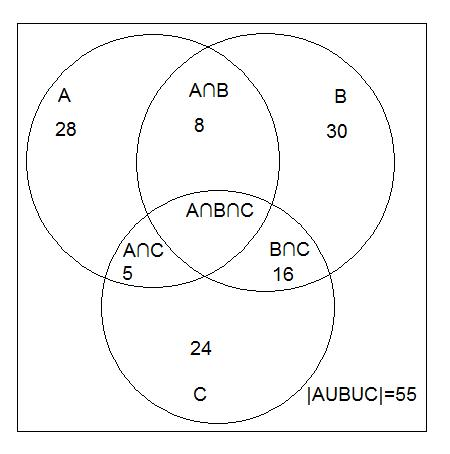
\includegraphics{venn}\\
\end{figure}
\noindent {\it Solution.} Let $A,B,C$ denote the set of students in algebra, biology, and chemistry class, respectively. Then $A\cup B\cup C$ is the set of students in one of the three classes, $A\cap B$ is the set of students in both algebra and biology, and so forth. To count the number of students in all three classes, i.e. count $|A\cup B\cup C|$, we can first add all the number of students in all three classes:
\[
|A|+|B|+|C|.
\]
However, now we've counted the students in two classes too many times. So we subtract out the students who are in each pair of classes:
\[
-|A\cap B|-|B\cap C|-|A\cap C|.
\]
For students who are in two classes, we've counted them twice, then subtracted them once, so they're counted once. But for students in all three classes, we counted them 3 times, then subtracted them 3 times. Thus we need to add them again:
\[
+|A\cap B\cap C|.
\]
Thus
\begin{align*}
|A\cup B\cup C|&=|A|+|B|+|C|-|A\cap B|-|B\cap C|-|A\cap C|+|A\cap B\cap C|\\
55&=28+30+24-8-16-5+|A\cap B\cap C|.
\end{align*}
Thus $|A\cap B\cap C|=2$, i.e. there are 2 students in all three classes.\\

The same reasoning works with an arbitrary number of sets; we state the general result in the following theorem.
\begin{thm}[Principle of Inclusion and Exclusion (PIE)]
 Let $A_1,\ldots, A_n$ be sets. Define $S_k=\sum_{1\le i_1<\cdots < i_k\le n} |A_{i_1}\cap \cdots \cap A_{i_k}|$,  %; abbreviate $[n]=\{1,2,\ldots, n\}$.
i.e. $S_k$ is a sum over all choices of $k$ subsets. For $k=1$, it's simply \[
|A_1|+|A_2|+|A_3|+\cdots+|A_k|
\]  
and for $k=n$, it represents one sum,
\[
|A_{1}\cap A_{2}\cap A_{3}\cap \cdots \cap A_{n}|.
\]  

Then
\begin{align*}
|A_1\cup \cdots \cup A_n|&=S_{1}-S_{2}+S_{3}+\cdots+(-1)^{n-1}S_{n}.
%\sum_{k=1}^n \sum_{1\le i_1\le \cdots \le i_k\le n}(-1)^{k} |A_{i_1}\cap \cdots \cap A_{i_k}|\\
%&=\sum_{1\le i_1\le i_2}|A_{i_1}|-\sum_{1\le i_1<i_2\le n}|A_{i_1}\cap A_{i_2}|+ \sum_{1\le i_1<i_2<i_3\le n}|A_{i_1}\cap A_{i_2}\cap A_{i_3}|-\cdots\\
%&\quad+(-1)^{n+1}|A_1\cap \cdots \cap A_n|.
\end{align*}
\end{thm}
\begin{proof}
Consider an element $x\in A_1\cup \cdots \cup A_n$. It is counted once on the left hand side, so we need to show that it is counted once on the right hand side as well. Suppose $x$ is in the sets $A_{j_1},\ldots, A_{j_m}$, but not in the rest of the sets. There are $\binom mk$ sets $\{i_1,\ldots, i_k\}$ such that $x\in A_{i_1}\cap \cdots \cap A_{i_k}$, since $\{i_1,\ldots, i_k\}$ has to be a subset of $\{j_1,\ldots,j_m\}$. Thus $x$ is counted $\binom mk$ times in the sum $\sum_{1\le i_1<\cdots <i_k\le n}|A_{i_1}\cap \cdots \cap A_{i_k}|$, and hence is counted
\[
\binom m1-\binom m2+\cdots +(-1)^{m-1}\binom mm
\]
on the right hand side. By the Binomial Theorem, $1-\binom m1+\binom m2-\cdots +(-1)^{m}\binom mm=(1-1)^m$, so 
\[
\binom m1-\binom m2+\cdots +(-1)^{m-1}\binom mm=1,
\]
showing $x$ is counted once in the RHS. If $x\nin A_1\cup \cdots \cup A_n$, clearly $x$ is not counted in either the LHS or the RHS. Since each element is counted the same number of times on either side, the theorem follows.
\end{proof}
\begin{ex}
Find the number of positive integers less than or equal to 1000 that are divisible by 7, 10, or 15.
\end{ex}
{\it Solution.} For a positive integer $k$, let $A_k$ denote the set of integers in $\{1,2,\ldots, 1000\}$ that are divisible by $k$. We want to find $|A_7\cup A_{10}\cup A_{15}|$. Note that
\[
A_k=\fl{\frac {1000}k}
\] 
where $\fl{y}$ denotes the greatest integer less than or equal to $y$. Indeed, the multiples of $k$ that are less than $1000$ are exactly $k, 2k,\ldots, \fl{\frac{1000}{k}}k$. Note also that $A_k\cap A_{\ell}=A_{\lcm(k,\ell)}$ since a number is divisible by both $k$ and $\ell$ if and only if it is divisible by $\lcm(k,\ell)$. Using PIE, we get
\begin{align*}
|A_7\cup A_{10}\cup A_{15}|&=|A_7|+|A_{10}|+|A_{15}|-|A_7\cap A_{10}|-|A_7\cap A_{15}|-|A_{10}\cap A_{15}|+|A_{7}\cap A_{10}\cap A_{15}|\\
&=|A_7|+|A_{10}|+|A_{15}|-|A_{70}|-|A_{105}|-|A_{30}|+|A_{210}|\\
&=\fl{\frac{1000}{7}}+\fl{\frac{1000}{10}}+\fl{\frac{1000}{15}}-\fl{\frac{1000}{70}}-\fl{\frac{1000}{105}}-\fl{\frac{1000}{30}}+\fl{\frac{1000}{210}}\\
&=142+100+83-14-9-33+4\\
&=273.
\end{align*}

Suppose instead we want to find the sum of positive integers satisfying the above properties, not the number of positive integers. What do we do? We replace each term $|S|$ in the sum above by $\sum_{x\in S} x$, so, rather than contributing $1$ to the value $S$, $x$ contributes the value $x$ to $S$. This is an example of the following more generalized version of inclusion-exclusion.
\begin{thm}
Let $f:A_1\cup \cdots \cup A_n\to \R$ be a function. Then
\begin{align*}
\sum_{x\in A_1\cup \cdots \cup A_n} f(x)&=\sum_{k=1}^n \sum_{1\le i_1< \cdots < i_k\le n}(-1)^{k} \sum_{x\in A_{i_1}\cap \cdots \cap A_{i_k}}f(x)\\
&=\sum_{1\le i_1\le n}\sum_{x\in A_{i_1}}f(x)-\sum_{1\le i_1<i_2\le n}\sum_{x\in A_{i_1}\cap A_{i_2}}f(x)+\cdots+(-1)^{n-1}\sum_{x\in A_1\cap \cdots \cap A_n} f(x).
\end{align*}
\end{thm}
Note that taking $f$ to be identically 1, we get the original statement of PIE.
\begin{proof}
The proof is the same as above, except now an element $x$ contained in $m$ of the sets contributes $f(x)$ to the left hand side and $\pa{\binom m1-\binom m2+\cdots +(-1)^{m+1}\binom mm}f(x)$ to the right hand side.
\end{proof}
\section{Permutations and surjections}
\begin{ex}
As $n$ people walk into a dinner party, they remove their hats. When they leave, the hats are randomly returned to them, so that all $n!$ matchings between people and hats are equally likely.

What is the probability that nobody gets his or her own hat back?
\end{ex}
\noindent {\it Solution.}
Labeling the people and the hats $1,2,\ldots, n$, a matching between people and hats corresponds to a permutation $\pi$ on $1,2,\ldots, n$, where $\pi(i)=j$ if person $i$ receives person $j$'s hat. 
So an equivalent formulation is the following: Given a random permutation 
on $\{1,2,\ldots, n\}$ (that is, a one-to-one function on $\{1,2,\ldots, n\}$), what is the probability that there is no fixed point, i.e. no $i$ such that $\pi(i)=i$?

Let $A$ be the set of permutations having a fixed point, and $D$ be the set of permutations having no fixed point (these permutations are called {\it derangements}).
We need to find $|A|$. To use PIE, we want to express $A$ as a union of sets whose sizes are easy to calculate. Note that $\pi$ having a fixed point means either 1 is a fixed point, or 2 is a fixed point, or 3 is a fixed point, or so on. Hence
\[
A=A_1\cup \cdots \cup A_n.
\]
where $A_i$ is the set of permutations $\pi$ such that $i$ is a fixed point, i.e. $\pi(i)=i$. By PIE, we have
\begin{equation}\label{hateq1}
|A|=\sum_{k=1}^n \sum_{1\le i_1<\ldots< i_k\le n} (-1)^{k-1} |A_{i_1}\cap \cdots \cap A_{i_k}|.
\end{equation}
An element $\pi$ of $A_{i_1}\cap \cdots \cap A_{i_k}$ must have $\pi(i_1)=i_1,\ldots, \pi(i_k)=i_k$, but can permute the other $n-k$ elements in any way. Hence 
\[
|A_{i_1}\cap \cdots \cap A_{i_k}|=(n-k)!
\]
Since there are $\binom nk$ sets of size $k$,~(\ref{hateq1}) becomes
\begin{align*}
|A|&=\sum_{k=1}^n (-1)^{k-1}\binom nk (n-k)!=\sum_{k=1}^n \frac{(-1)^{k-1}}{n!}{k!}\\
|D|&=n!-|A|=\sum_{k=0}^n \frac{(-1)^{k}n!}{k!}.
\end{align*}

Thus the desired probability is
\[
\frac{|D|}{n!}=\sum_{k=0}^n \frac{(-1)^{k}}{k!}.
\]

Readers familiar with calculus may recognize that truncated series for $\rc{e}$ appears above:
\[
\rc{e}=1-\rc{1!}+\rc{2!}-\rc{3!}+\rc{4!}-\cdots 
\]
We calculated that
\[
|D|=n!\pa{1-\rc{1!}+\rc{2!}-\cdots \frac{(-1)^{n}}{n!}}.
\]
Hence
\[
|D|-\frac{n!}{e}=n!\sum_{k=n+1}^{\iy} \frac{(-1)^k}{k!}\in \pa{-\frac{n!}{(n+1)!},\frac{n!}{(n+1)!}}\subeq \pa{-\rc 2,\rc 2}.
\]
Hence $|D|$ equals $\frac{n!}{e}$ rounded to the nearest integer, i.e. $|D|=\fl{\frac{n!}{e}+\frac{1}{2}}$ and the probability equals
\[
p=\fl{\frac{1}{e}+\frac{1}{2n!}}.
\]
In particular, as the number of hats $n$ goes to infinity, the probability that all people get their hats back approaches $\rc e$.

Note: What makes this proof so fascinating, is that it shows us whether it's five people who derange their hats or a thousand or billion, it will generally be the same probability. 

\begin{ex}
Suppose $m\ge n$. Find the number of surjective functions $f:\{1,2,\ldots, m\}\to \{1,2,\ldots, n\}$, i.e. functions $f$ such that $f(x)=k$ has a solution for any $k\in \{1,2,\ldots, n\}$.
\end{ex}
\noindent{\it Solution.}
Let $S$ be the set of surjective functions. 
As in the previous example, we find it more convenient to consider the complement of the desired set, then subtract it from the set of all functions. 
So let $A=S^c$ be the set of non-surjective functions.
We can express $A$ as a union
\[
A=A_1\cup \cdots \cup A_n
\]
where $A_k$ is the set of functions $f:\{1,2,\ldots, m\}\to \{1,2,\ldots, n\}$ whose range does not include $k$. Then by PIE,
\begin{equation}\label{nonsurjeq1}
|A|=\sum_{k=1}^{n}\sum_{1\le i_1<\cdots <i_k\le n} (-1)^{k+1} |A_{i_1}\cap \cdots \cap A_{i_k}|.
\end{equation}

Now $|A_{i_1}\cap \cdots \cap A_{i_k}|$ consists of all functions that miss the values $i_1,\ldots, i_k$. This leaves $n-k$ possibilities for each of $f(1),\ldots, f(m)$, so there are $(n-k)^m$ such functions. Since there are $\binom nk$ subsets of size $k$,~(\ref{nonsurjeq1}) becomes
\[
|A|=\sum_{k=1}^n (-1)^{k-1}\binom nk (n-k)^m.
\]
Since there are $n^m$ functions from $\{1,\ldots, m\}$ to $\{1,\ldots, n\}$, we get
\[
|S|=n^m-\sum_{k=1}^n (-1)^{k-1}\binom nk (n-k)^m
=\sum_{k=0}^n (-1)^{k}\binom nk (n-k)^m.
\]


%\section{Sieves in Number Theory}
%In number theory, we often want to estimate the number of integers in a given range having certain divisibility properties, for example, we want to estimate the number of primes, or the number of twin primes.
%%For instance, if $P$ is a set of primes, we may want to estimate the number $m$ of integers between $0$ and $n$ that are relatively prime to all elements of $P$. Following example~(), we know by PIE that
%%\[
%%m=x-\sum_{p_1\le x}\fl{\frac xp}+\sum_{p_2\le x}\fl
%%\]
%
%In this section, we use sieve methods to derive an upper bound for the $n$th twin prime. (A twin prime is a prime $p$ such that $p+2$ is also prime.)
%\begin{thm}
%Let $\pi_2(x)$ denote the number of twin primes less than or equal to $x$. Then
%\[
%\pi_2(x)\preceq \frac{x (\ln \ln x)^2}{(\ln x)^2}.
%\]
%\end{thm}
%Note we write $f(x)\preceq g(x)$ if there is a constant $c$ such that $f(x)\le cg(x)$ for sufficiently large $x$. Our bound says that twin primes are pretty sparse: the prime number theorem says that the number of primes less than or equal to $x$, $\pi(x)$, is asymptotically $\frac{x}{(\ln x)^2}$. The difference is enough so that the sum of the reciprocal of all primes diverges,
%\[
%\sum_{p\text{ prime}} \rc{p}=\iy,
%\]
%while the sum of the reciprocal of the twin primes converges.
%\[
%\sum_{p\text{ twin prime}} \rc{p}<\iy.
%\]
%(See Exercise ?).
%
%The first important observation is that $p$ is a twin prime if and only if $p(p+2)$ is a product of 2 primes.
\section{Problems}
\begin{enumerate}
\item (AHSME 1983/26) The probability that event $A$ occurs is $\frac 34$; the probability that event $B$ occurs is $\frac 23$. Let $p$ be the probability that both $A$ and $B$ occur. Find the smallest interval necessarily containing $p$.
\item At Sunnydale High School there are
\begin{itemize}
\item 44 students in either algebra, biology, or chemistry class
\item 25 students in biology class
\item 23 students in chemistry class
\item 13 students in both algebra and biology
\item 9 students in both biology and chemistry
\item 10 students in both algebra and chemistry
\item 6 students in all three classes.
\end{itemize}
How many students are in algebra class?
\item Four couples are sitting in a row. Find the number of arrangements in which no person is sitting next to his or her partner. What if they are sitting in a circle?
\item Find the number of five-digit combinations from the set $\{1,2,3,4,5\}$ in which:
\begin{enumerate}
\item
Some digit appears at least three times.
\item
No digit appears more than twice.
\end{enumerate}
\item Let $\{p_1,\ldots, p_r\}$ be a set of primes. Show that the number of positive integers less than or equal to $n$ and relatively prime to $p_1,\ldots, p_r$ is equal to
\[
x\pa{1-\rc{p_1}}\cdots \pa{1-\rc{p_r}}+2^r\theta
\]
for some $-1< \theta <1$.
\item Find the sum of all positive integers less than or equal to $1000$ that are not divisible by $7$, $10$, or $15$.
\item Find the number of solutions to
\[
x_1+x_2+x_3+x_4+x_5+x_6=15
\]
such that each $x_i$ is an integer and $0\le x_i\le 4$.
\item Specially marked boxes of ChocoBalls cereal contain one of four puzzle pieces, each with probability $\rc 4$. Once you have all four puzzle pieces, you can mail them in and receive a coupon for more ChocoBalls cereal.
\begin{enumerate}
\item
If Jim buys $n$ specially marked boxes of ChocoBalls cereal, what is the probability that he gets all four puzzle pieces?
\item
What is the expected number of boxes that Jim has to buy to get all four puzzle pieces?
\end{enumerate}
\item
Find the number of permutations $\pi$ of $\{1,2,\ldots, n\}$ such that $\pi(i+1)\ne \pi(i)+1$ for all $1\le i\le n$.
\item Let $a_n$ be the number of permutations $\pi$ of $\{1,2,\ldots, 2n\}$ such that $\pi(i+1)-\pi(i)\ne n$ for each $1\le i\le 2n-1$. Find $a_n$ and show that $\lim_{n\to \iy}\frac{a_n}{(2n)!}=\rc{e}$.
\item (TST 2004/2) Assume $n$ is a positive integer. Consider sequences $a_0,a_1,\ldots, a_n$ such that $a_i\in \{1,2,\ldots, n\}$ for each $i$ and $a_n=a_0$.
\begin{enumerate}
\item
Call such a sequence {\it good} if for all $i=1,2,\ldots, n$, $a_i-a_{i-1}\nequiv i\pmod n$. Suppose $n$ is odd. Find the number of good sequences.
\item
Call such a sequence {\it great} if for all $i=1,2,\ldots, n$, $a_i-a_{i-1}\nequiv i,2i\pmod n$. Suppose that $n$ is an odd prime. Find the number of great sequences.
\end{enumerate}
(Note: We solved this problem using generating functions and complex numbers in lecture 11. Try to do it with PIE this time.)
\item (IMO 1991/3) Let $S=\{1,2,3,\ldots, 280\}$. Find the minimal natural number $n$ such that in any $n$-element subset of $S$ there are five numbers that are pairwise relatively prime.
\item (USAMO 1994/5)
Let $|U|$, $\si(U)$, and $\pi(U)$ denote the number of elements, the sum, and the product, respectively, of a finite set $U$ of positive integers. (If $U$ is the empty set, $|U|=0$, $\si(U)=0$, and $\pi(U)=1$.) Let $S$ be a finite set of positive integers. As usual, let $\binom nk$ denote $\frac{n!}{k!(n-k)!}$. Prove that
\[
\sum_{U\subeq S} (-1)^{|U|} \binom{m-\si(U)}{|S|}=\pi(S)
\]
for all integers $m\ge \si(S)$.
\end{enumerate}
\begin{thebibliography}{9}
\bibitem{HK}The Inclusion-Exclusion Principle, 2011. \url{http://www.math.ust.hk/~mabfchen/Math232/Inclusion-Exclusion.pdf}
\end{thebibliography}
\end{document}